\section{Network Architecture and Methodology}
Recall that in our project, due to large variation in the axial axis, we specified our problem into 2D segmentation task.\\

\subsection{Unet}
%TODO describe Unet here
We implemented a 2D Unet model as the baseline model, the original Unet structure is described in \ref{tab:OriginalUnet}. We further added a Batch Normalization layer before each activation better to alleviate covariance shift. The input image channel is one in our case because CT volumes are grey scale images.\\

We selected the input as original size because we want to reserve as much detail as possible. 
The input dimension is then (batch-size $\times$ 1 $\times$ 512 $\times$ 512), and the output dimension after softmax is (batch-size $\times$ 2 $\times$ 512 $\times$ 512) for the binary segmentation task, and we take an argmax to get the binary image the same size as the input.\\

\begin{table}
\centering
	\begin{tabular}{l c c c}
	\hline
	\hline
	Layer	&	input	&	output	&	channel	\\
	\hline
	Conv 3x3 + RELU	&	572	&	570	&	64	\\
	Conv 3x3 + RELU	&	570	&	568	&	64	\\
	Max Pool 2 $\times$ 2	&	568	&	284	&	64	\\
	Conv 3x3 + RELU	&	284	&	282	&	128	\\
	Conv 3x3 + RELU	&	282	&	280	&	128	\\
	Max Pool 2 $\times$ 2	&	280	&	140	&	128	\\
	Conv 3x3 + RELU	&	140	&	138	&	256	\\
	Conv 3x3 + RELU	&	138	&	136	&	256	\\
	Max Pool 2 $\times$ 2	&	136	&	68	&	256	\\
	Conv 3x3 + RELU	&	68	&	66	&	512	\\
	Conv 3x3 + RELU	&	66	&	64	&	512	\\
	Max Pool 2 $\times$ 2	&	64	&	32	&	512	\\
	Conv 3x3 + RELU	&	32	&	30	&	1024	\\
	Conv 3x3 + RELU	&	30	&	28	&	1024	\\
	up-conv 2 $\times$ 2	&	28	&	56	&	512	\\
	convs 1x1	&	56	&	54	&	512	\\
	convs 1x1	&	54	&	52	&	512	\\
	up-conv 2 $\times$ 2	&	52	&	104	&	256	\\
	convs 1x1	&	104	&	102	&	256	\\
	convs 1x1	&	102	&	100	&	256	\\
	up-conv 2 $\times$ 2	&	100	&	200	&	128	\\
	convs 1x1	&	200	&	198	&	128	\\
	convs 1x1	&	198	&	196	&	128	\\
	up-conv 2 $\times$ 2	&	196	&	392	&	64	\\
	convs 1x1	&	392	&	390	&	64	\\
	convs 1x1	&	388	&	388	&	2	\\
	\hline
	\hline
	\end{tabular}
	\caption{The Original Unet Architechture}
	\label{tab:OriginalUnet}
\end{table}

\subsection{Attention Gated Unet}
%TODO Describe Attention gate here
We used the original Attention Gated Unet architecture recommended in the paper \cite{Attention_gate_network} that we added the Gate block before the skip connection concatenate to the upconvolution result in the corresponding layer.
An illustration is shown in figure \ref{fig:attention_gate}.
\begin{figure}
	\centering
	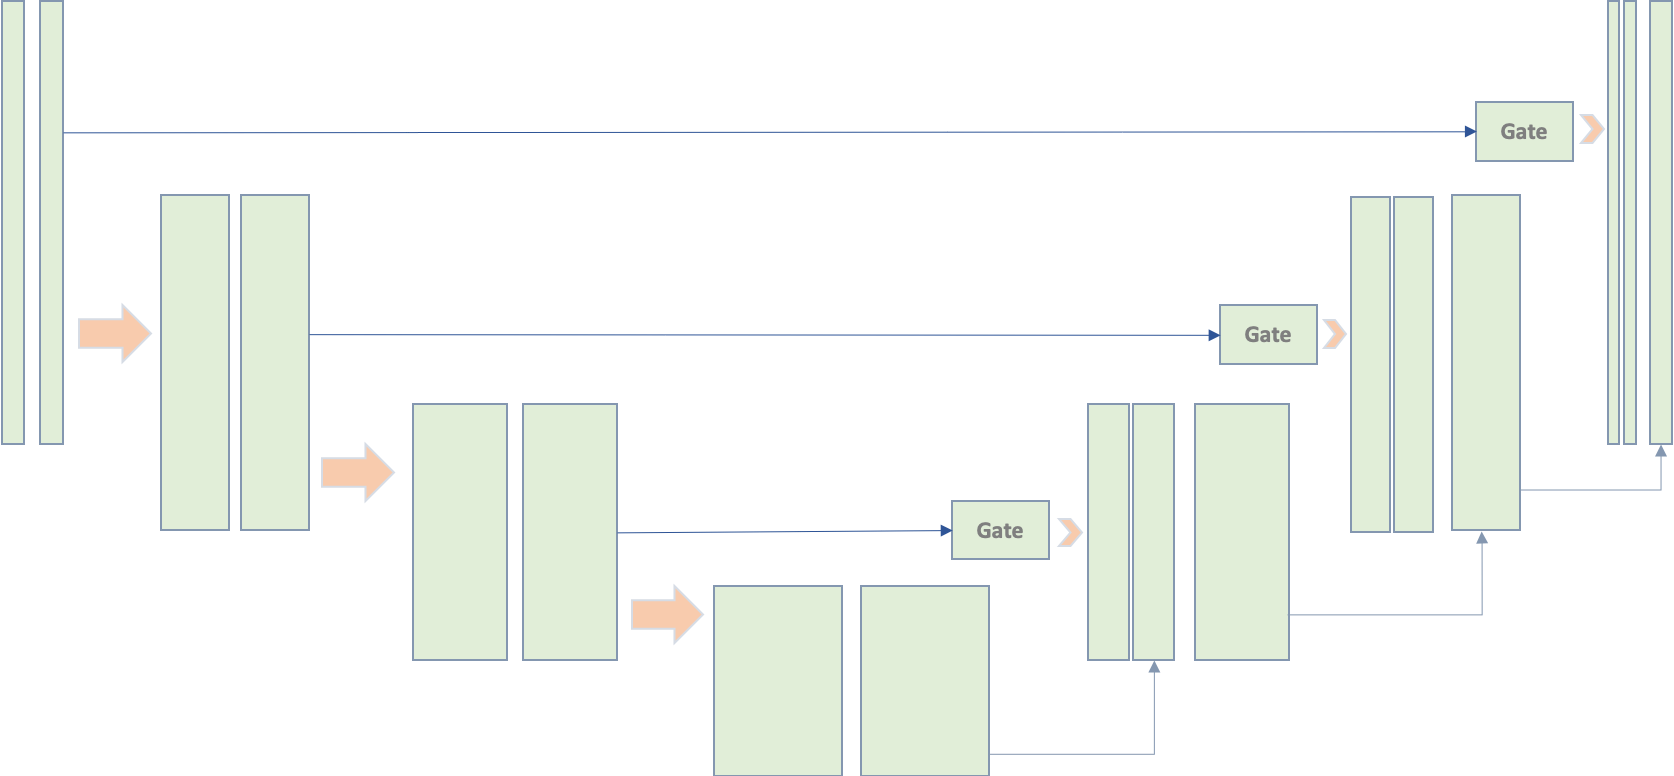
\includegraphics[width=0.8\textwidth]{img/Net_arch/attention_gate}
	\caption{An illustration of the attention block added in the Unet}	
	\label{fig:attention_gate}
\end{figure}

\subsection{Loss function}
\subsubsection{Training objectives}
In this project, we used a combination of Foreground Soft Dice loss and Cross Entropy Loss. The justification of these combination is:
\begin{itemize}
	\item We consider CE loss converge fast for the background to learn the rough location of the segmentation
	\item We consider Foreground Dice only because for our highly imbalanced segmentation problem, adding background will vanish the loss and our segmentation target will not learn well.
\end{itemize}
Mathematically, we write our objective function as:
$$Loss=\frac{1}{I} \sum_{i=1}^{I} 1-\frac{2 \sum_{l=1}^{L} \sum_{c=1}^{C} p_{l}^{c} r_{l}^{c}}{2 \sum_{l=1}^{L} \sum_{c=1}^{C} p_{l}^{c}+r_{l}^{c}} - -\frac{1}{N} \sum_{c=1}^{N} \frac{1}{w_{c}} \sum_{l=1}^{L} r_{l}^{c} \log \left(p_{l}^{c}\right)$$

\subsubsection{Validation and testing scenario}
For Validating or testing the network, we used the foreground hard Dice Loss calculating the range of overlap.
$$Dice Loss = \frac{2|A \cap B|}{|A|+|B|}$$

\subsection{Transfer Learning}
As we discussed in the background chapter, the pretrained network from a source domain can serve as a good starting point for the issue especially when training data is not that sufficient. We make use of the initialized weights trained on our own  and fine tune the model on both the plain Unet and Attention Unet.
\begin{figure}
	\centering
	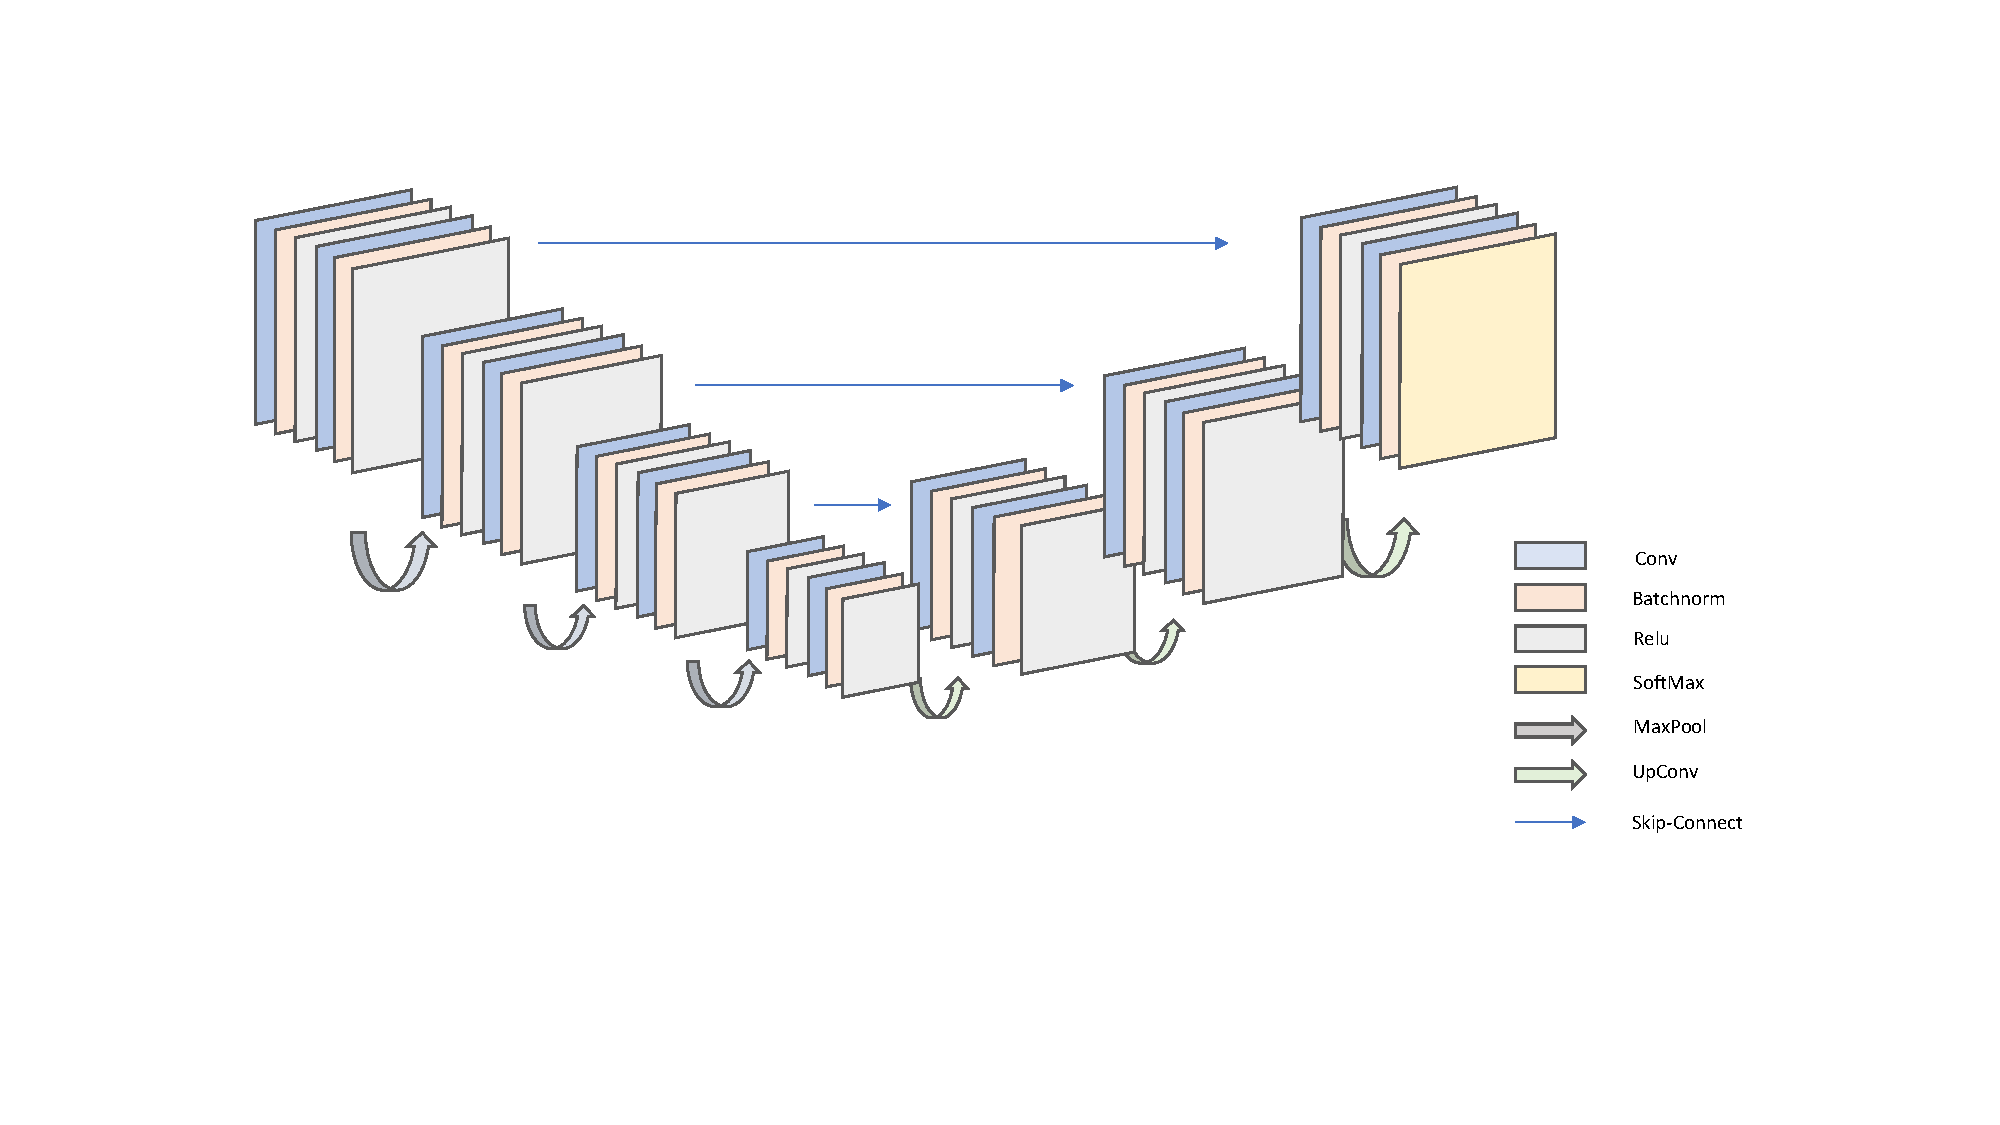
\includegraphics[width=0.8\textwidth]{img/Networks/Unet-train.pdf}
	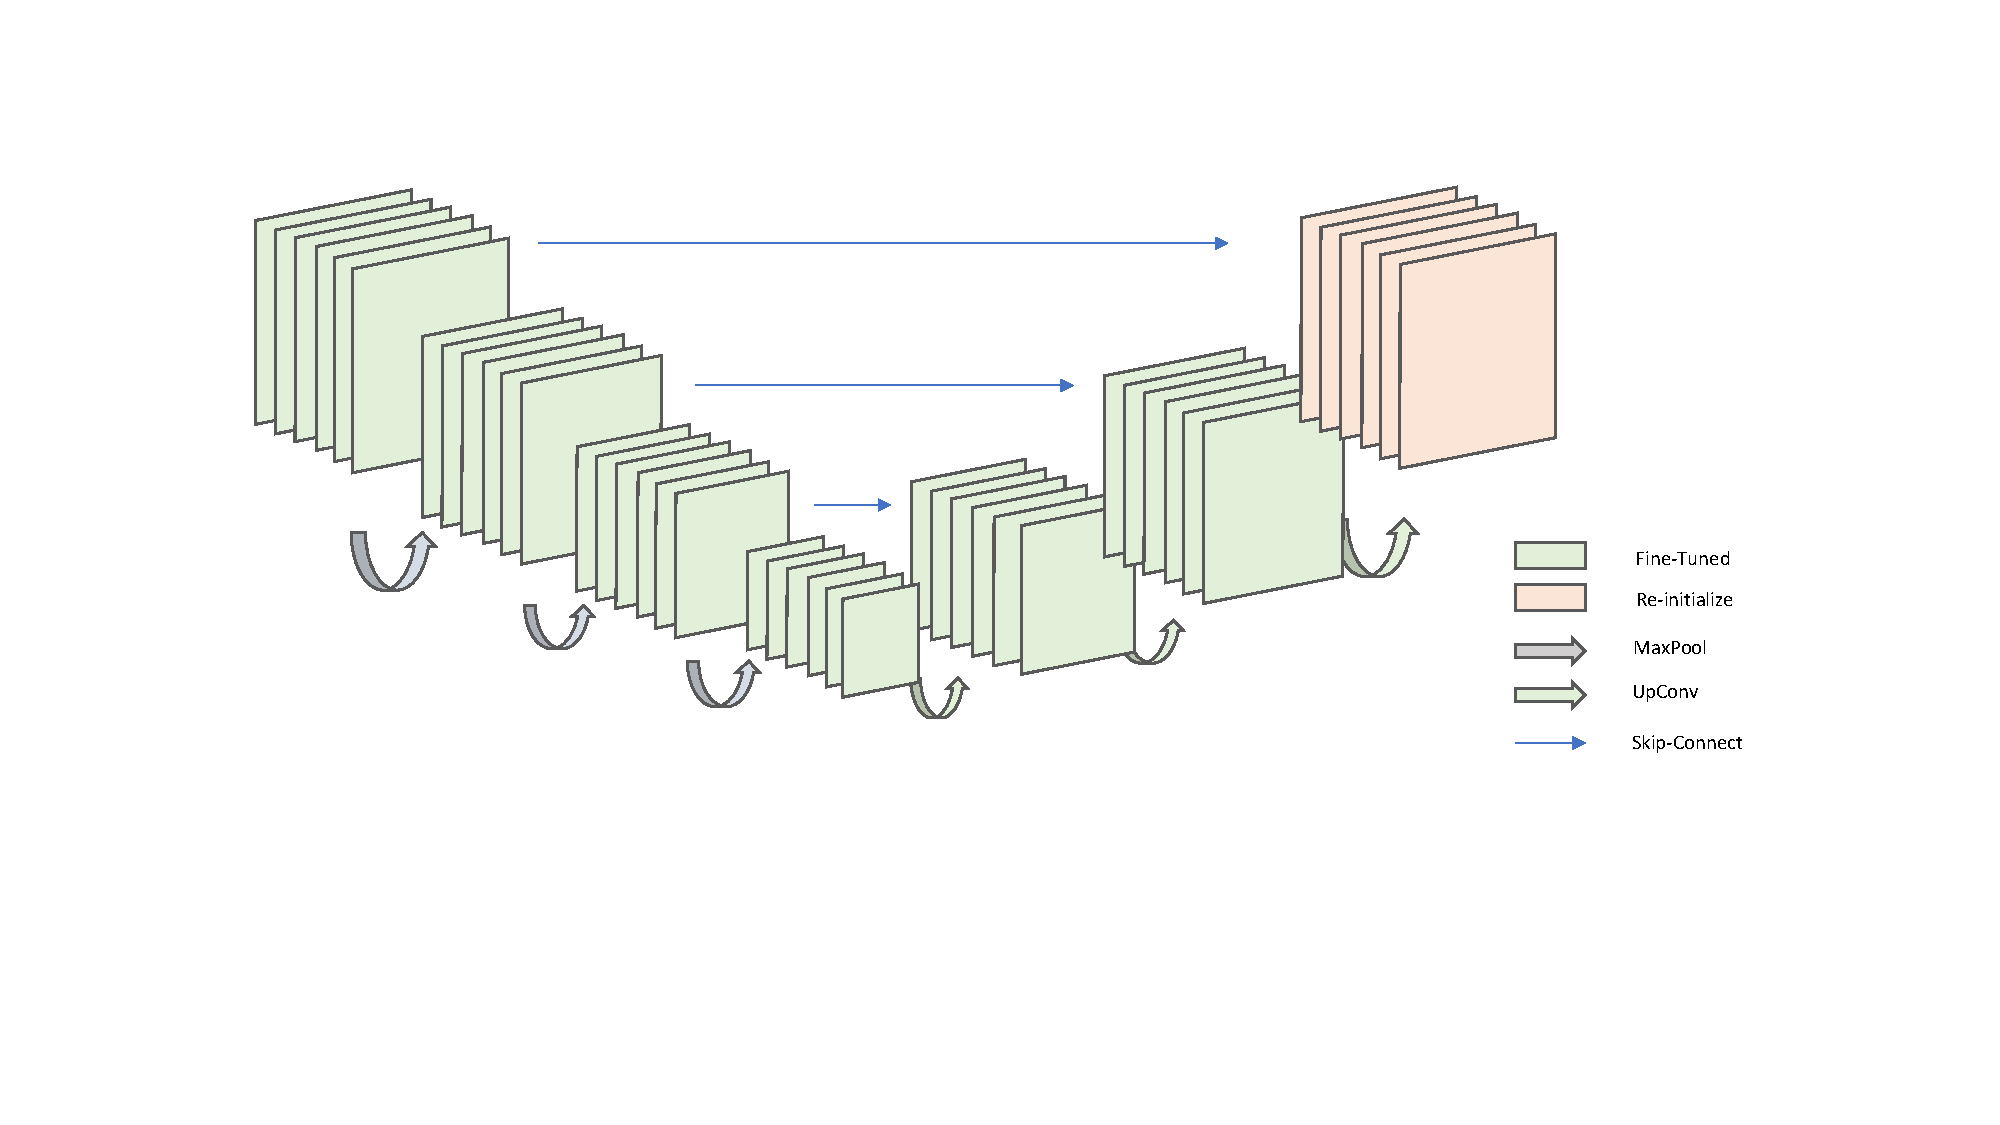
\includegraphics[width=0.8\textwidth]{img/Networks/Transfer-Finetune-all.pdf}
	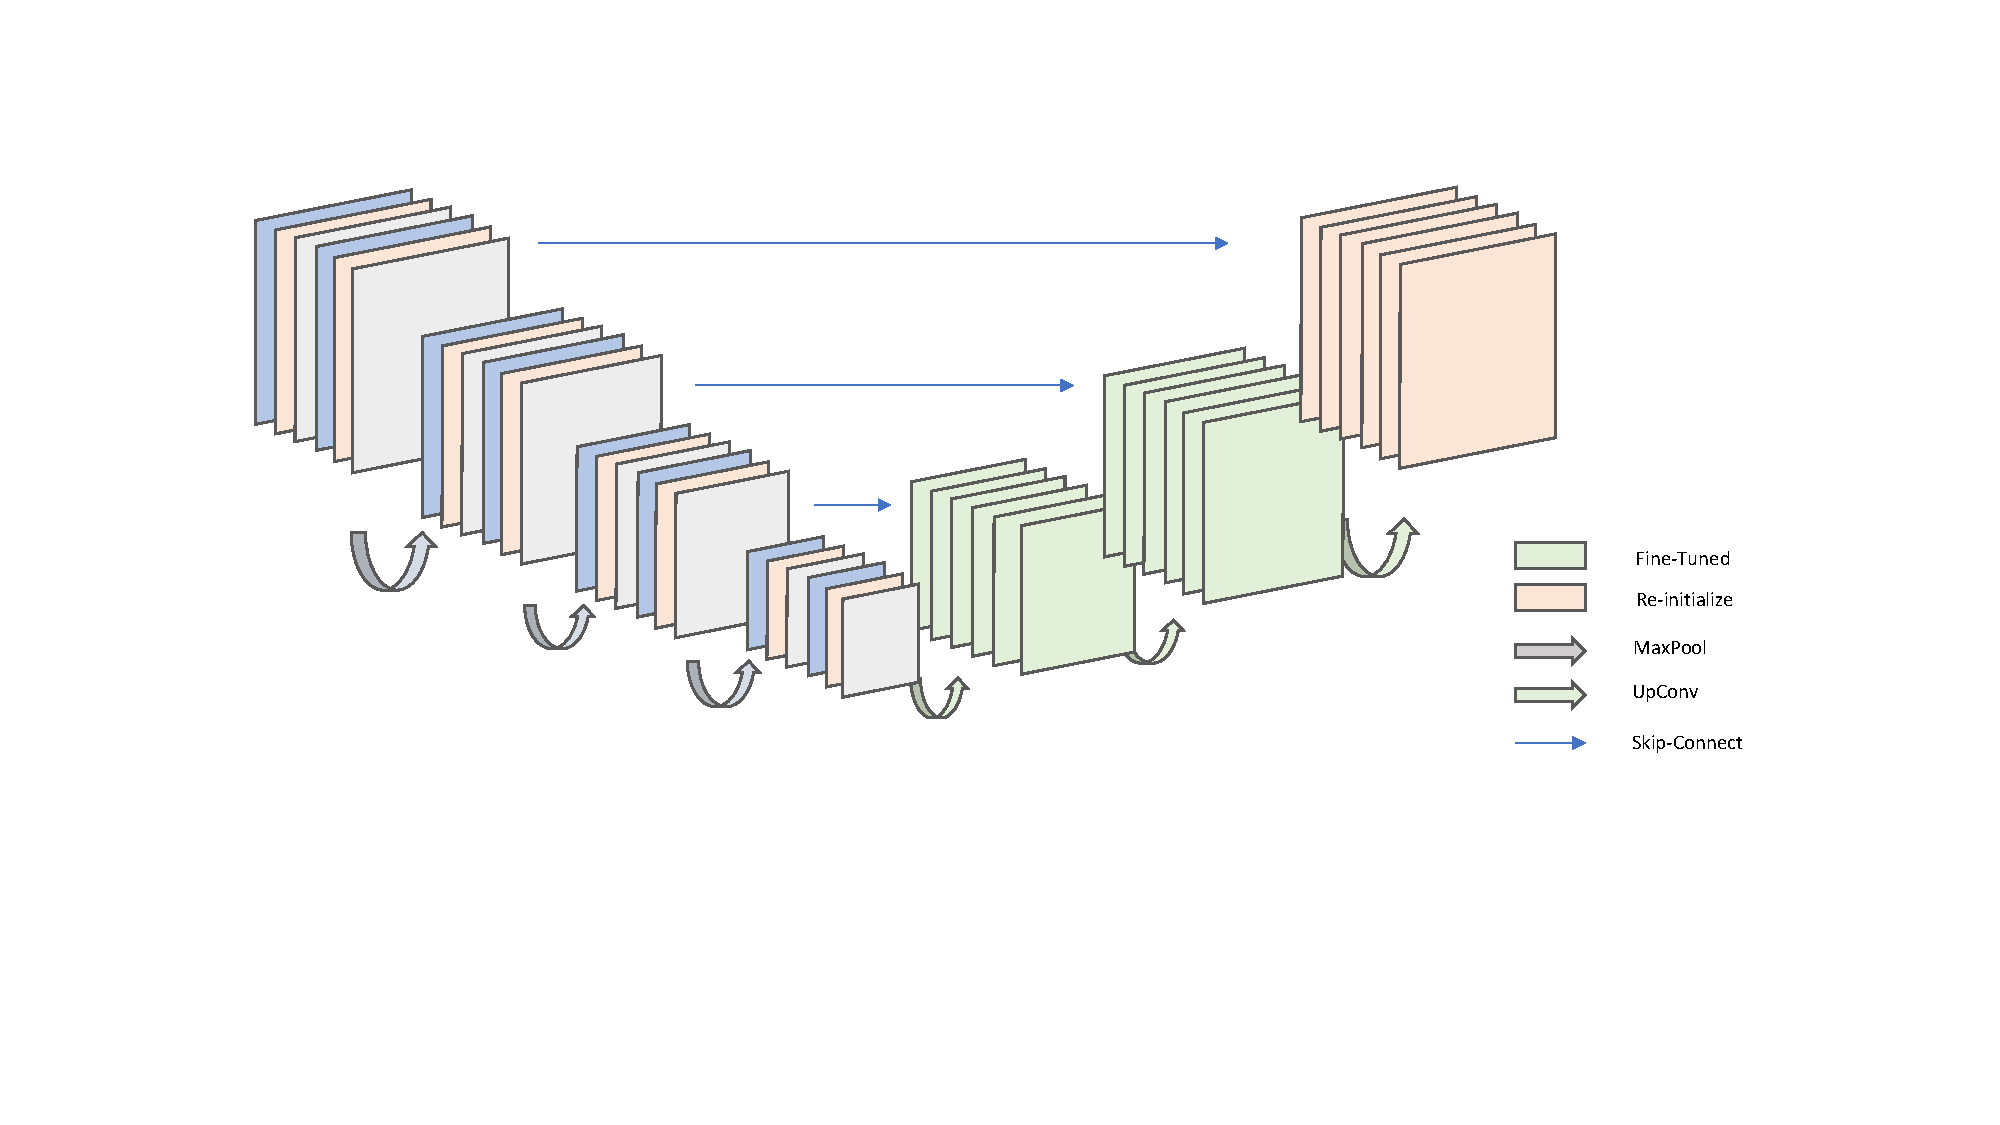
\includegraphics[width=0.8\textwidth]{img/Networks/Transfer-freeze-encoder.pdf}
	\caption{An illustration of Network structure used for pretraining and transfer-learning}
	\label{fig:transfer-learning-graph}
\end{figure}

\subsubsection{Pretraining}
For pretraining, we leverage two model initializations. We pretrained the model with the mixed Non-Covid lung Dataset, and we also used the weight initialization of the Model Genesis Dataset.
We pretrained the segmentation model using non-Covid dataset based on the assumption that the weights serves as good starting point for the fine-tuning stage.
	
\subsubsection{Fine-Tuning}
We fine tuned the two pre-trained model using both of the initialization to train the Unet and the Attention Gate Unet architecture. We did experiment that allow the network to fine tune all or we freeze the encoder part. The justification of freezing the encoder can be further explained in the experiment section that SVCCA showed that the encoder showed less movement during fine-tuning.

\begin{enumerate}
	\item Freeze encoder: We freeze the first half of the encoder, and fine tuned the decoder except that we re-initialized the output layer.
	\item Fine-Tune-All: The whole network is fine tuned and the last block of convolutional layers was reinitialized.
\end{enumerate}

\begin{itemize}
	\item Fine-Tuning Unet: We directly load the trained model from the image and train the network and did the experiment with the two Fine-Tuning methods mentioned above.
	\item Fine-tuning Attention Gate: We consider that the attention gate for different domain are different, so for both of the fine-tuning methods, we take the encoder part only and append new decoder and attention gate to train from scratch.
\end{itemize}


\section{SVCCA implementation}
%TODO insert SVCCA implementaiton here
For the implementation in our work, we followed the tutorial\footnote{https://github.com/google/svcca/tree/master/tutorials} in paper \cite{raghu_svcca_2017}.\\

Recall from the background section that SVCCA evaluates the aligned similarity of two sets of output feature maps across the feature channels.\\
\begin{itemize}
	\item Throughout the training we saved the model every 100 epochs if the validation accuracy reports higher compared to the previous validation, such as the model during training at epoch 100 vs the converged model we saved at the end of the training.  Our experiments focus on same layers between two models.
	\item For each model, we hooked the \textbf{layer activation output} over the entire validation set (2D images).
	\item Then we load the two output into two numpy arrays with dimension [num\_data, channel, height, width]. 
	\item We flatten the data into two 2D arrays with dimension [channel, num\_data * height * width] so that we keep the channel wise difference. The justification of this step is that each pixel in the feature map  sees a different area (receptive field, shown in figure) in the original image.
	\item Then we perform singular value decomposition (SVD) so that the output subspace directions keeps 99\% of the original variance。
	\item We then compute Canonical Correlation similarity analysis (CCA) on the output subspace which transform the subspace for maximum alignment then compute the correlation coefficients $\rho$. The SVCCA score is the average of the coefficients $\bar {\rho}$.
\end{itemize}
 
\begin{figure}
	\centering
	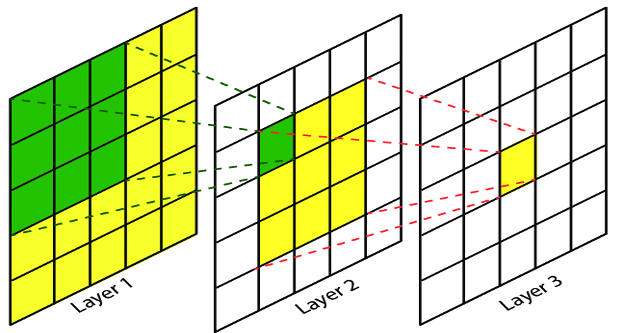
\includegraphics[width=0.5\textwidth]{img/Net_arch/receptive_field}
	\caption{Receptive field illustration}
\end{figure}

\section{Designed semi-supervise pipeline}
Given that a larger amount of unlabelled data was published later in our project, we further investigated the semi-supervise segmentation area leveraging unlabelled dataset. \textbf{We constructed a semi-supervise learning framework including pseudo labeling, and mean-teacher training with our loss function.} The whole pipeline is shown in figure 

\begin{figure}[h]
	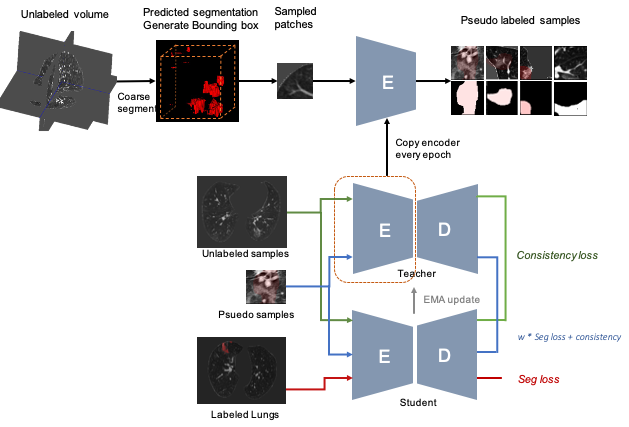
\includegraphics[width=\textwidth]{img/Net_arch/semi-arch}
	\caption{An overview of the proposed semi-supervise pipeline}
\end{figure}

\subsection{Pseudo labeling}
We developed a new pseudo labeling framework that assign a reasonable label to the unlabelled samples.\\

We sampled both the labelled samples and the unlabelled images. For the labeled samples, we first get the bounding box of the segmentation mask, then enlarge the mask by a maximum of 10 pixels each side, and we sampled images within that bounding box.
For unlabeled images, we use the coarse 3D segmentation to generate the bounding box, and the bounding box was enlarged maximum of 15 pixels, we sample patches within the coarse bounding box.
To assign a noisy psuedo label to the cropped images, we take the encoder part of the trained 2D segmentation model and append a Global Average Pooling function. We then encode a dictionary of the annotated samples in the feature space.\\
\begin{figure}
	\centering
	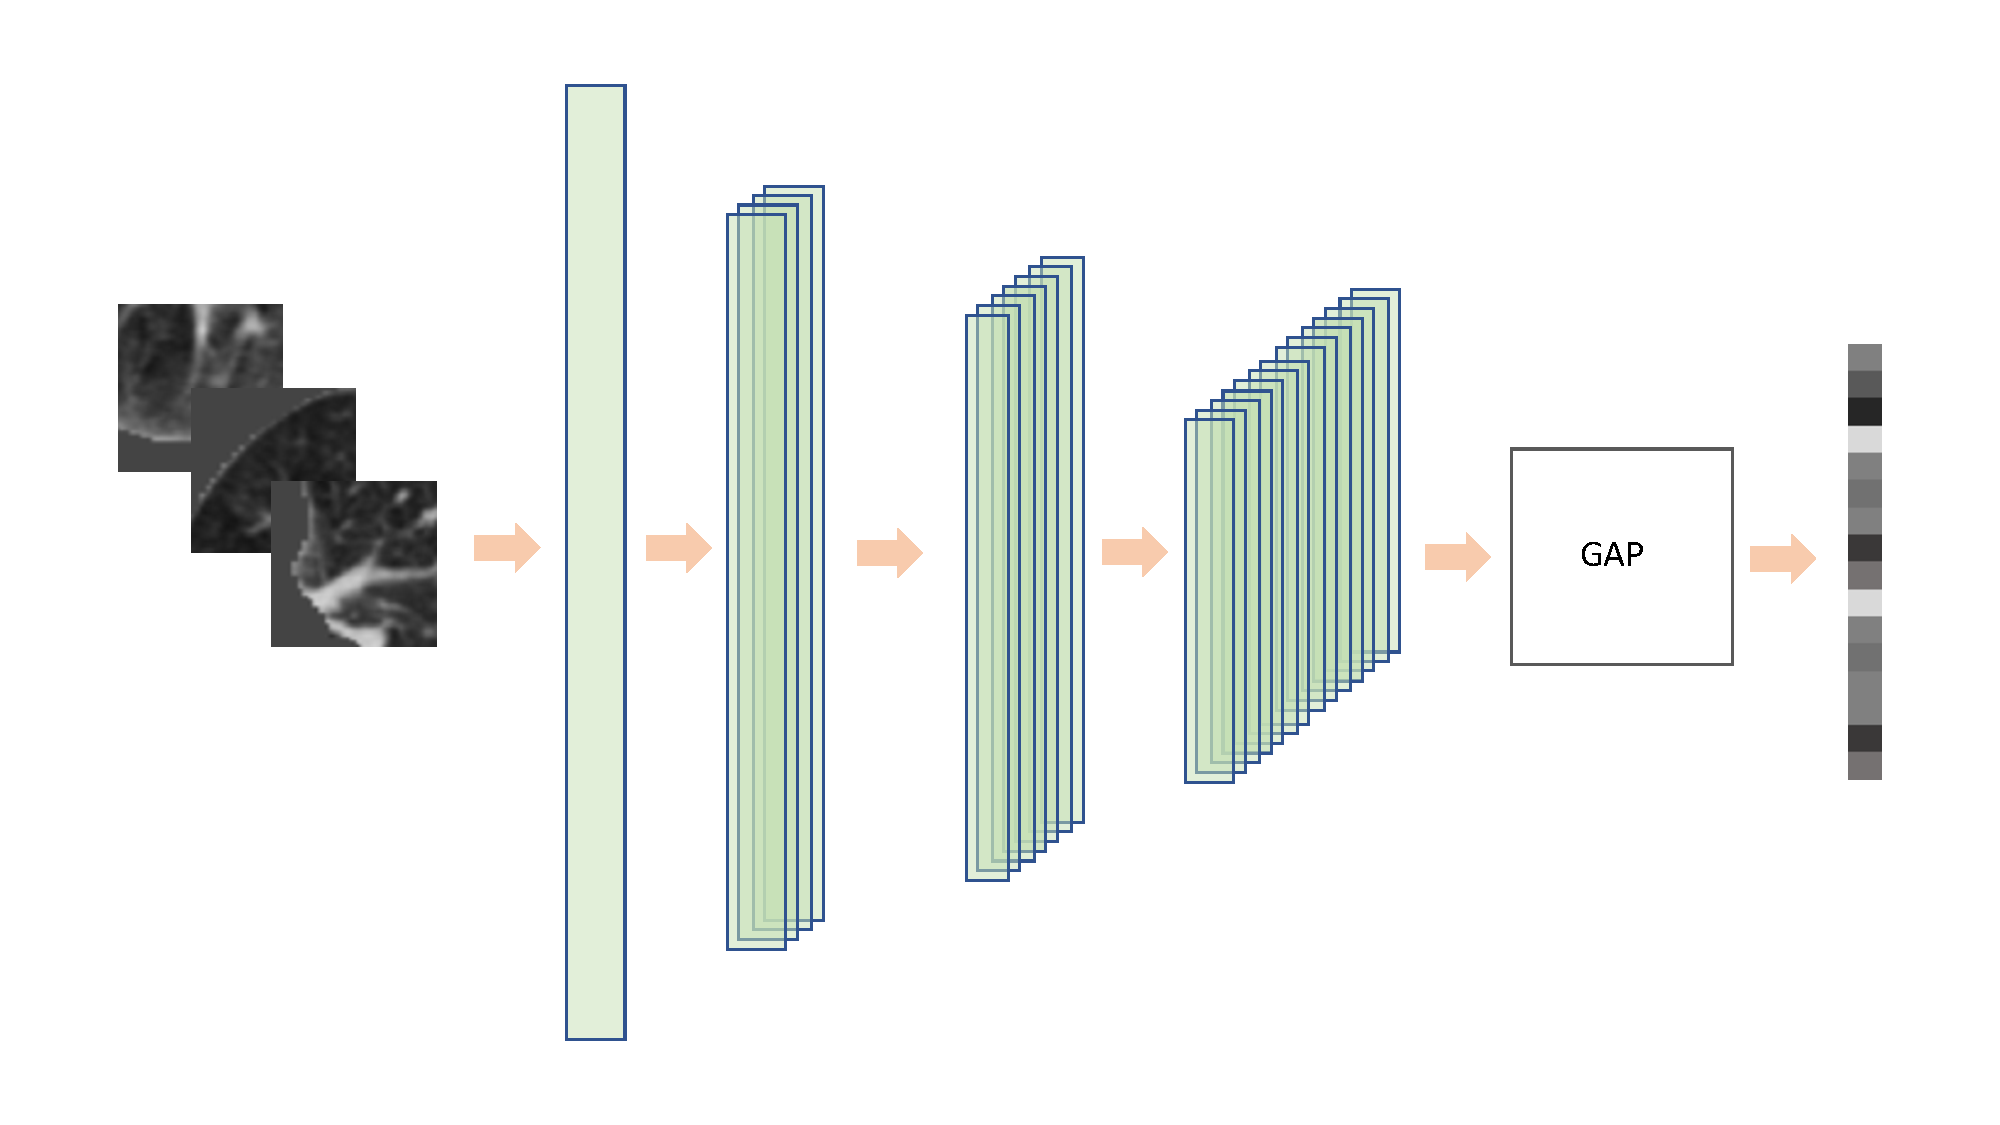
\includegraphics[width=0.9\textwidth]{img/semi-experiment/latent-space}
	\caption{An illustration of feature encoding process}
\end{figure}

For assigning noisy pseudo labels, given an unlabeled sample $I_{unlabeled}$ and its latent representation $Latent(I_{unlabelled})$, we calculated the pairwise cosine similarity and return the maximum cosine similarity score as the weight for this sample. 
$$\operatorname{similarity}(A, B)=\frac{A \cdot B}{\|A\| \times\|B\|}=\frac{\sum_{i=1}^{n} A_{i} \times B_{i}}{\sqrt{\sum_{i=1}^{n} A_{i}^{2}} \times \sqrt{\sum_{i=1}^{n} B_{i}^{2}}}$$
An illustration of the label assigning process is shown in figure \ref{fig:semi-label-assign}\\

\begin{figure}
	\centering
	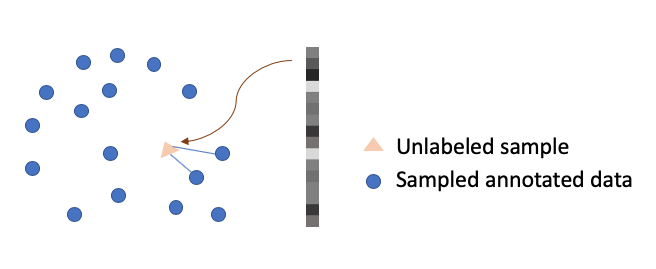
\includegraphics[width=0.8\textwidth]{img/semi-experiment/semi-label-assign}
	\caption{An illustration of label assigning to unlabelled samples}
	\label{fig:semi-label-assign}
\end{figure}

\subsection{Designed Architecture}
After assigning reasonable psuedo labels to the samples, as we described in Chapter 2, we designed a Mean-teacher style model for the semi-supervise task.\\

The teacher model is the 2D UNet we described in section 4.1 transferred using the non-covid dataset because we found that transfer learning give a better result as a initialization (detail in chapter 5), except that we only update the weight for no more than 10 epochs because we want the teacher model to be a bit more noisy than the converged model.\\

We first copied the trained weights to get the student model. 
For updating weights, we let the pseudo-labeled patch go through the teacher and student model, and calculate the prediction consistency, as well as a degraded dice score on the student network prediction. We set the weight to  Similarity score * Dice Loss for a lighter penalization. We then let the labelled patches go through the student model and calculate the prediction error with $Loss = Dice + CE$ (detail in next section). The student network weights are updated using back propagation each iteration. Teacher network is updated though an exponential moving average. During validation, we validate on both of the models and observe the performance.                    

 Figure \ref{fig:mean-teacher-training} showed an illustration of the weight update process using this framework.
 %TODO insert here the formal loss function
\begin{figure}[h]
	\centering
	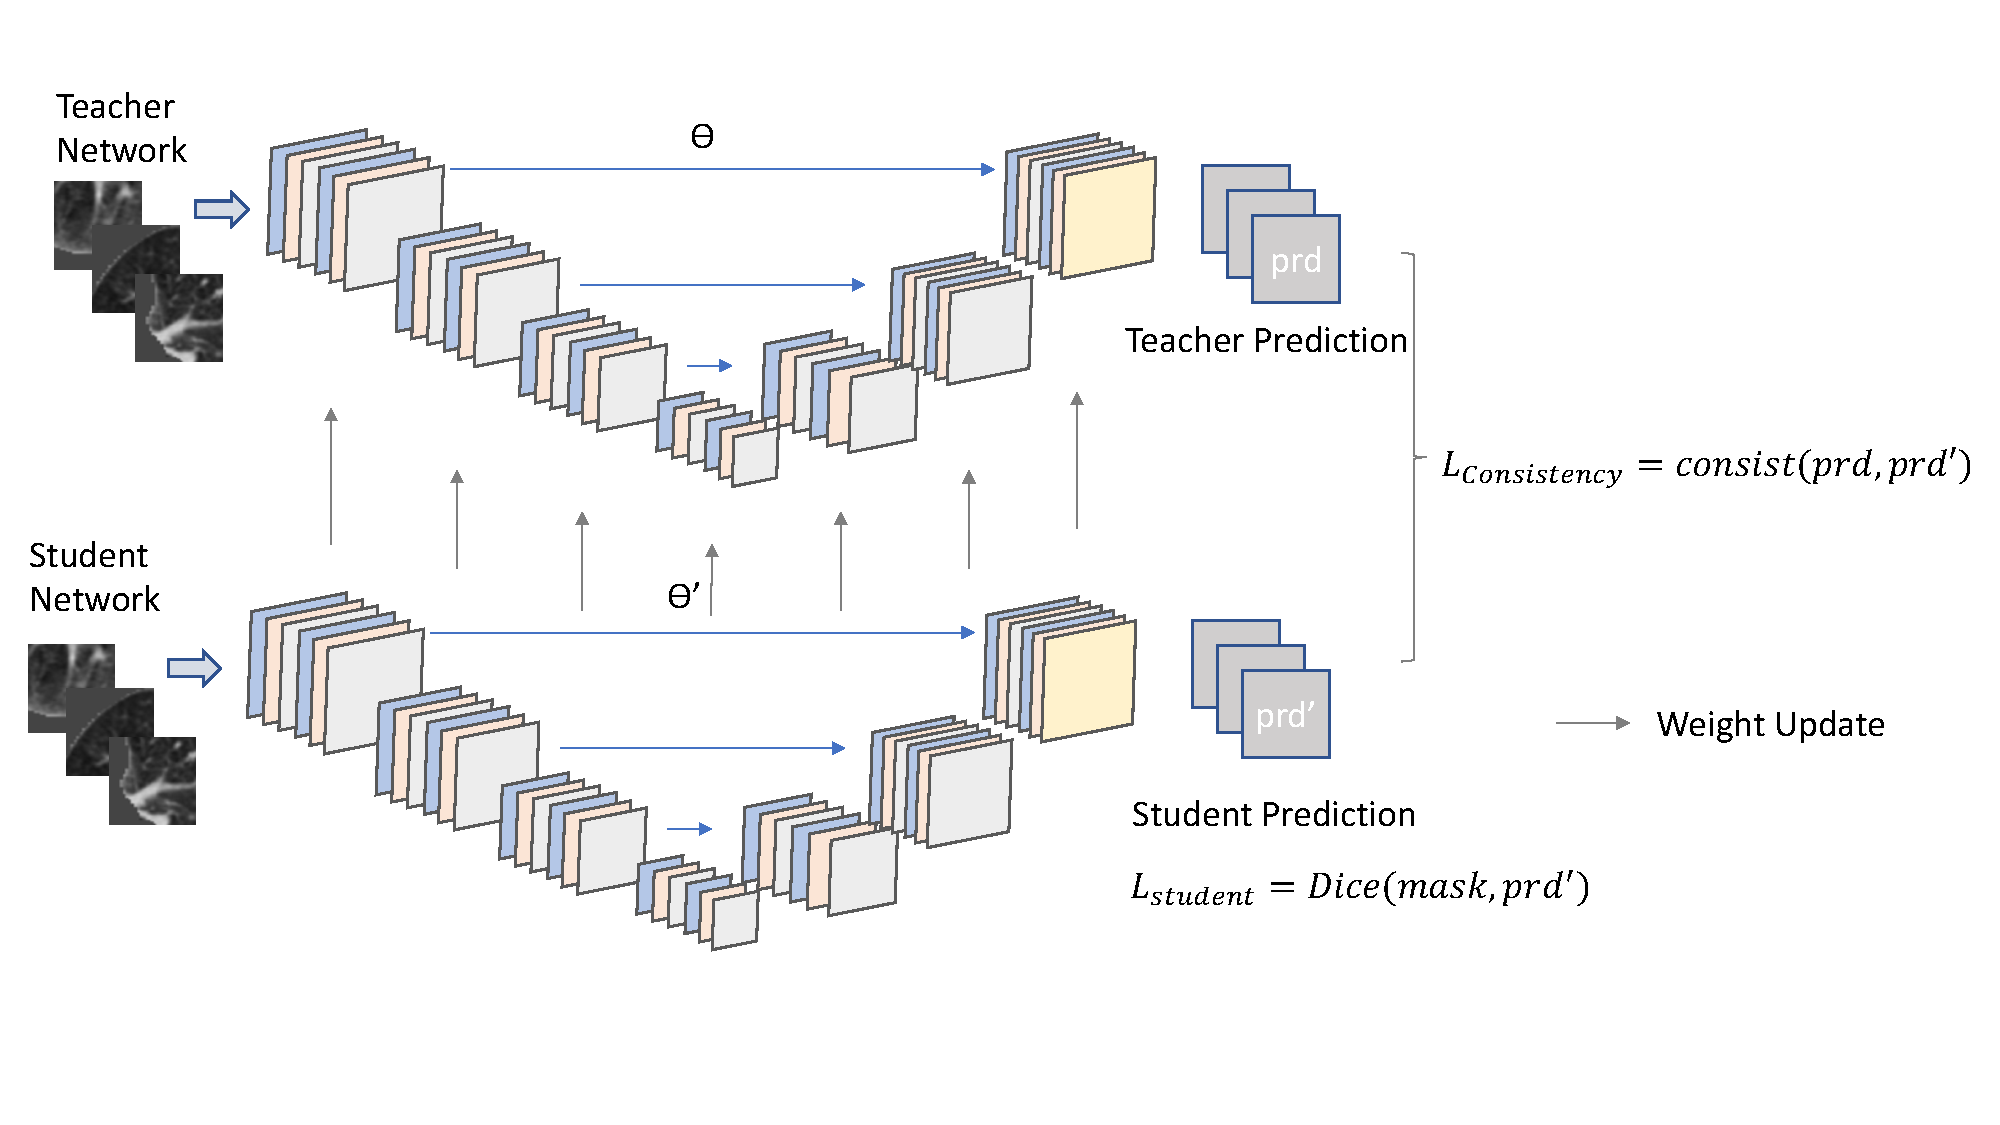
\includegraphics[width=\textwidth]{img/Networks/mean-teacher-net}
	\caption{The design of network model for our semi-supervise setup}
	\label{fig:mean-teacher-training}
\end{figure}

\subsection{Loss function for training}
Mathematically, we write the Loss function as

$$L_{labeled-train} = L_{segmentation} = Dice(prd_{student}, seg) + CE(prd_{student}, seg)$$ 
$$L_{unlabeled-train} = CE(prd_{teacher}, prd_{student}) + weight * Dice(prd_{student}, mask) $$
\subsection{Validation and testing}
For the evaluation, we used the Dice Loss as we did in section 4.1.

